\documentclass{beamer}
\usepackage[export]{adjustbox}
\usepackage{theme/DM}

\title{DM Beamer Template}
\subtitle{DM Beamer Template Subtitle}
\author{Unknown Author}
\institute{Data Mining Lab, UESTC}
\logo{
    \raisebox{-50pt}[0pt][0pt]{
        
\includegraphics[decodearray={0.8 1 0.8 1 0.8 1},width=0.5\textwidth,left=0.4\textwidth]{theme/dmlogo.png}
    }
}

\begin{document}

\begin{frame}[plain]
    \titlepage
\end{frame}

\begin{frame}
    \tableofcontents[sectionstyle=show,subsectionstyle=show/shaded/hide,subsubsectionstyle=show/shaded/hide]
\end{frame}

\section{Section 1}

% \subsection{Subsection 1}

\begin{frame}
    \frametitle{Test}
    \framesubtitle{Subtitle Test}
    This is some text in the first frame. This is some text in the first frame. This is some text in the first frame.
\end{frame}

\begin{frame}
    \frametitle{Test}
    This is a text in second frame.
    For the sake of showing an example.

    \begin{itemize}
        \item<1-> Text visible on slide 1
        \item<2-> Text visible on slide 2
        \item<3> Text visible on slide 3
        \item<4-> Text visible on slide 4
    \end{itemize}
\end{frame}

\section{Section 2}

\begin{frame}
    \frametitle{Test}
    In this slide, some important text will be
    \alert{highlighted} because it's important.
    Please, don't abuse it.

    \begin{block}{Remark}
        Sample text
    \end{block}

    \begin{alertblock}{Important theorem}
        Sample text in red box
    \end{alertblock}

    \begin{examples}
        Sample text in green box. The title of the block is ``Examples".
    \end{examples}
\end{frame}

\begin{frame}
    \frametitle{Test}
    \begin{center}
        \begin{tabular}{|l|c|}\hline
            J.\ S.\ Bach   & 1685--1750 \\
            W.\ A.\ Mozart & 1756--1791 \\
            L.\ Beethoven  & 1770--1827 \\
            F.\ Chopin     & 1810--1849 \\
            R.\ Schumann   & 1810--1856 \\
            B.\ Bart\'{o}k & 1881--1945 \\ \hline
        \end{tabular}
    \end{center}
\end{frame}

\begin{frame}
    \frametitle{Two Column Output}
    \begin{columns}[c]
        \column{0.5\linewidth}
        Practical \TeX\ 2005\\
        Practical \TeX\ 2005\\
        Practical \TeX\ 2005
        \column{0.5\linewidth}
        \framebox{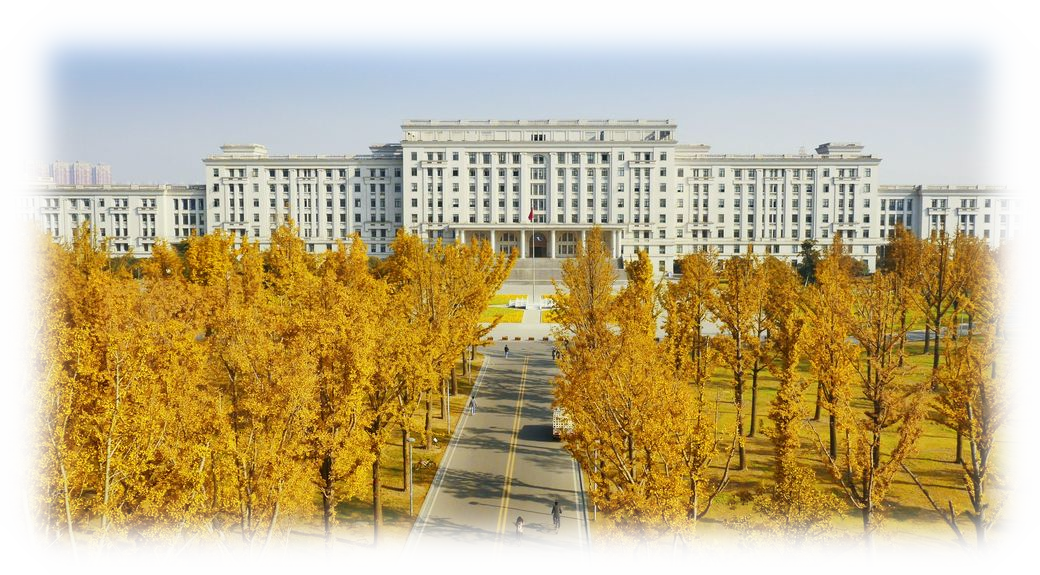
\includegraphics[width=1.5in]{theme/uestcscene.png}}
    \end{columns}
\end{frame}

\begin{frame}
    \Huge Thanks!
\end{frame}

\end{document}


